%----------------------------------------------------------------------------
\chapter{A poros plazma kísérlet}
%----------------------------------------------------------------------------
\section{Bevezető}
	A poros plazma kísérlet ionizált nemesgáz és az abba szórt porrészecskék megfigyeléséből áll.
	Adott alacsony nyomású gáz terében elhelyezett elektródákra kapcsolt váltakozó feszültséggel 
	lehetséges plazmát létrehozni. A váltakozó villamos tér a töltéssel rendelkező elektronokra 
	olyan erővel hat, hogy azok leszakadnak az atomról ezzel ionizálva azokat.
	A leszakadó elektronok a térben szabadon a ráható erőknek megfelelően mozognak.
	Ez makroszkópikus skálán a gáz vezetővé válását jelenti. A szabad elektronok mozgásának
	során az ionizált atomokon szórodnak, ami ködfénykisüléshez vezet. 
	
	A kísérlet során az előbb ismertett plazma terébe porrészecskéket szórunk. A porrészecskék alatt
	$10nm - 100\mu m$ nagyságú részecskéket értünk, például $SiO_2$, $Al_2O_3$ vagy 
	melamine-formaldehyde-t. A porrészecskék a plazmával interakcióba lépve negatívan feltöltődnek.
	A porrészecskék töltésének és tömegének hányadosa a szabad elektronokhoz és az ionokhoz képest
	sokkal kissebb, ezáltal a mozgására való hatása elhanyagolható.
	
	A porrészecskék transzportjának megértéséhez szükséges a ráható erők azonosítása.
	A különféle erők nagysága a porrészecskék nagyságától különféleképpen skálázódik. Elhanyagolásokat
	ennek megfelelően tehetünk.
	\begin{description}
		\item[Gravitációs $F_g$ erő:] Mikrógravitációban végzett kísérletek kivételével a porrészecskére
			ható gravitációs erő lineárisan arányos a tömegével. Nanométer nagyságú részecskék esetén
			elhanyagolható, de a jelen esetben használt mikrométer nagyságú részecskék esetén dominánsak,
		\item[Villamos tér keltette $F_e$ erő:] A porrészecske töltésével és a villamos tér nagyságával
			arányos. A megfelelően irányított villamos térrel lehetséges a részecskék levitációja,  
		\item[Háttératomon való szóródás $F_n$:] A porrészecske driftje során a háttératomokkal való
			szóródásának makroszkópikus erőként való számításba vétele,
		\item[Hőmérséklet grandiensi $F_{th}$ erő:] A gáz hőmérsékletének gradiense okozta
			gázatomok diffúzív jellegű mozgása által okozott indirekt erőhatás,
		\item[Ion sudrási $F_i$ erő:] Az ionokra ható villamos tér okozta erőnek indirekt hatása a
			porrészecskékre.
	\end{description}
	A poros plazma analízise során fontos szerepet játszik a részecskék csatolása.
	A csatolást gyengének és erősnek kategorizáljuk aszerint, hogy a részecskék szomszédja általi
	átlagos potenciális energia az átlagos termikus energiához képest kissebb vagy nagyobb.
	A csatolást a Coulomb csatolási paraméterrel ($\Gamma$) lehet számosítani, ami a szomszédos
	részecskék Coulomb potenciáljának és termikus energiájának hatványa:
	\begin{equation}
		\Gamma = \cfrac{Q^2 / 4\pi\varepsilon_0 d}{kT_d} 
	\end{equation}
	ahol $Q$ a részecskék töltése, $d$ az átlagos részecske távolság és a $T_d$ a por hőmérséklete.
	Ha a $\Gamma$ értéke egy kritikus érték fölé $\Gamma > 150$ növekszik, akkor
	porrészecskék Coulomb kristályszerkezetbe rendeződik.
	
	Az iparban anyag porlasztására és mintázat maratására használják. Továbbá szennyeződésként a VLSI
	áramkörök gyártásakor jelentkezik, ami kihozatal csökkenését és a teljesítmény csökkenéséhez vezet.

%----------------------------------------------------------------------------
\section{A kísérlet}
%----------------------------------------------------------------------------
	A kísérlet lebonyolítására egy speciális kamrára van szükség, amiben lehetséges a plazma
	létrehozása, a porrészecskék szórása illetve a megfelelő villamos tér létrehozása.
	A kamrának hermetikusan jól zártnak kell lennie, hogy csak a kívánt gázt tartalmazza.
	A középvákuumú működéshez kétlépéses vákuumszivattyút kell alkalmazni.
	
	\begin{figure}[!h]
		\centering
		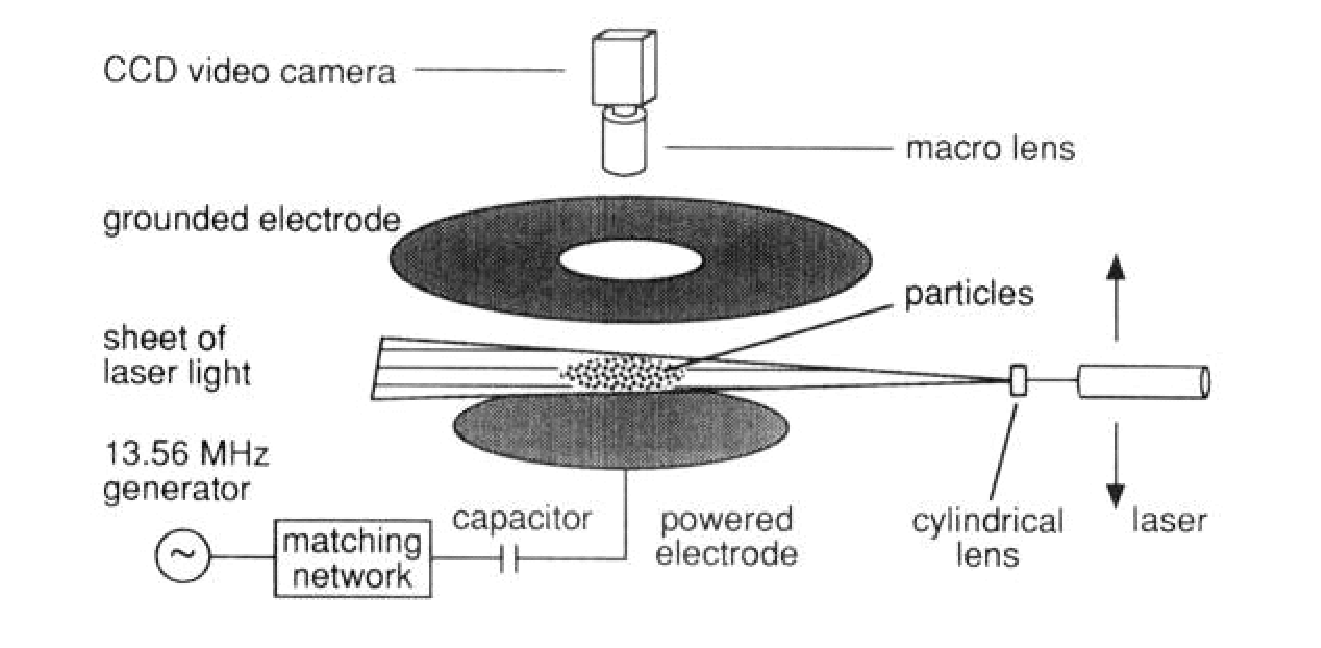
\includegraphics[width=0.9\columnwidth]{figures/eps/dust_camera.eps}
		\caption{A mérési elrendezés sematikus ábrája (forrás: \cite{Merlino2006})} 
		\label{fig:meresch} 
	\end{figure}
	
	A kamra sematikus ábrája a \ref{fig:meresch}. ábrán látható.
	A porrészecskék levitációjáért a villamos tér felelős. Az 1D síkba való zárás parabolikus
	potenciállal lehetséges. Az ilyen tér létrehozása a következő elektródákkal lehetséges: alul
	elhelyezett korong alakú elektróda, ami felett egy gyűrű alakú elektróda helyezkedik el.
	Az ilyen elektródarendszerre kapcsolt váltakozó feszültség a beszórt porrészecskéket lebegtetni
	tudja. Továbbá a részecskék követéséhez lézerrel megvilágítjuk és nagysebességű kamerával
	felvételt készítünk róla.
	
	A konkrét kamra paraméterei:
	\begin{itemize}
		\item Kamra belső átmérője $25cm$
		\item Kamra belső magassága $18cm$
		\item Alsó elektróda átmérője $18cm$
		\item Felső gyűrű elektróda belső átmérője $15cm$
		\item Felső elektróda távolsága az alsótól $13cm$
		\item Argon gáz nyomása $1.2\pm0.05 Pa$
		\item Gáz átfolyása $\sim 0.01 CCPM$
		\item Váltakozó feszültség $7W\quad @ \quad 13.56 MHz$
		\item Porrészecske: melamine-formaldehyde
		\item Porrészecske átmérője $4.38\pm 0.06 \mu m$
		\item Porrészecske tömege $6.64\cdot10^{-14} kg$
		\item Látható porrészecskék száma $\sim 2500$
		\item Megvilágító lézer: $200mW\quad @ \quad 532nm$
		\item Kamera $1.4MPixel$
	\end{itemize}
	Ilyen felvétel látható a \ref{fig:measurement}. ábrán. 	
	
	\begin{figure}[!h]
		\centering
		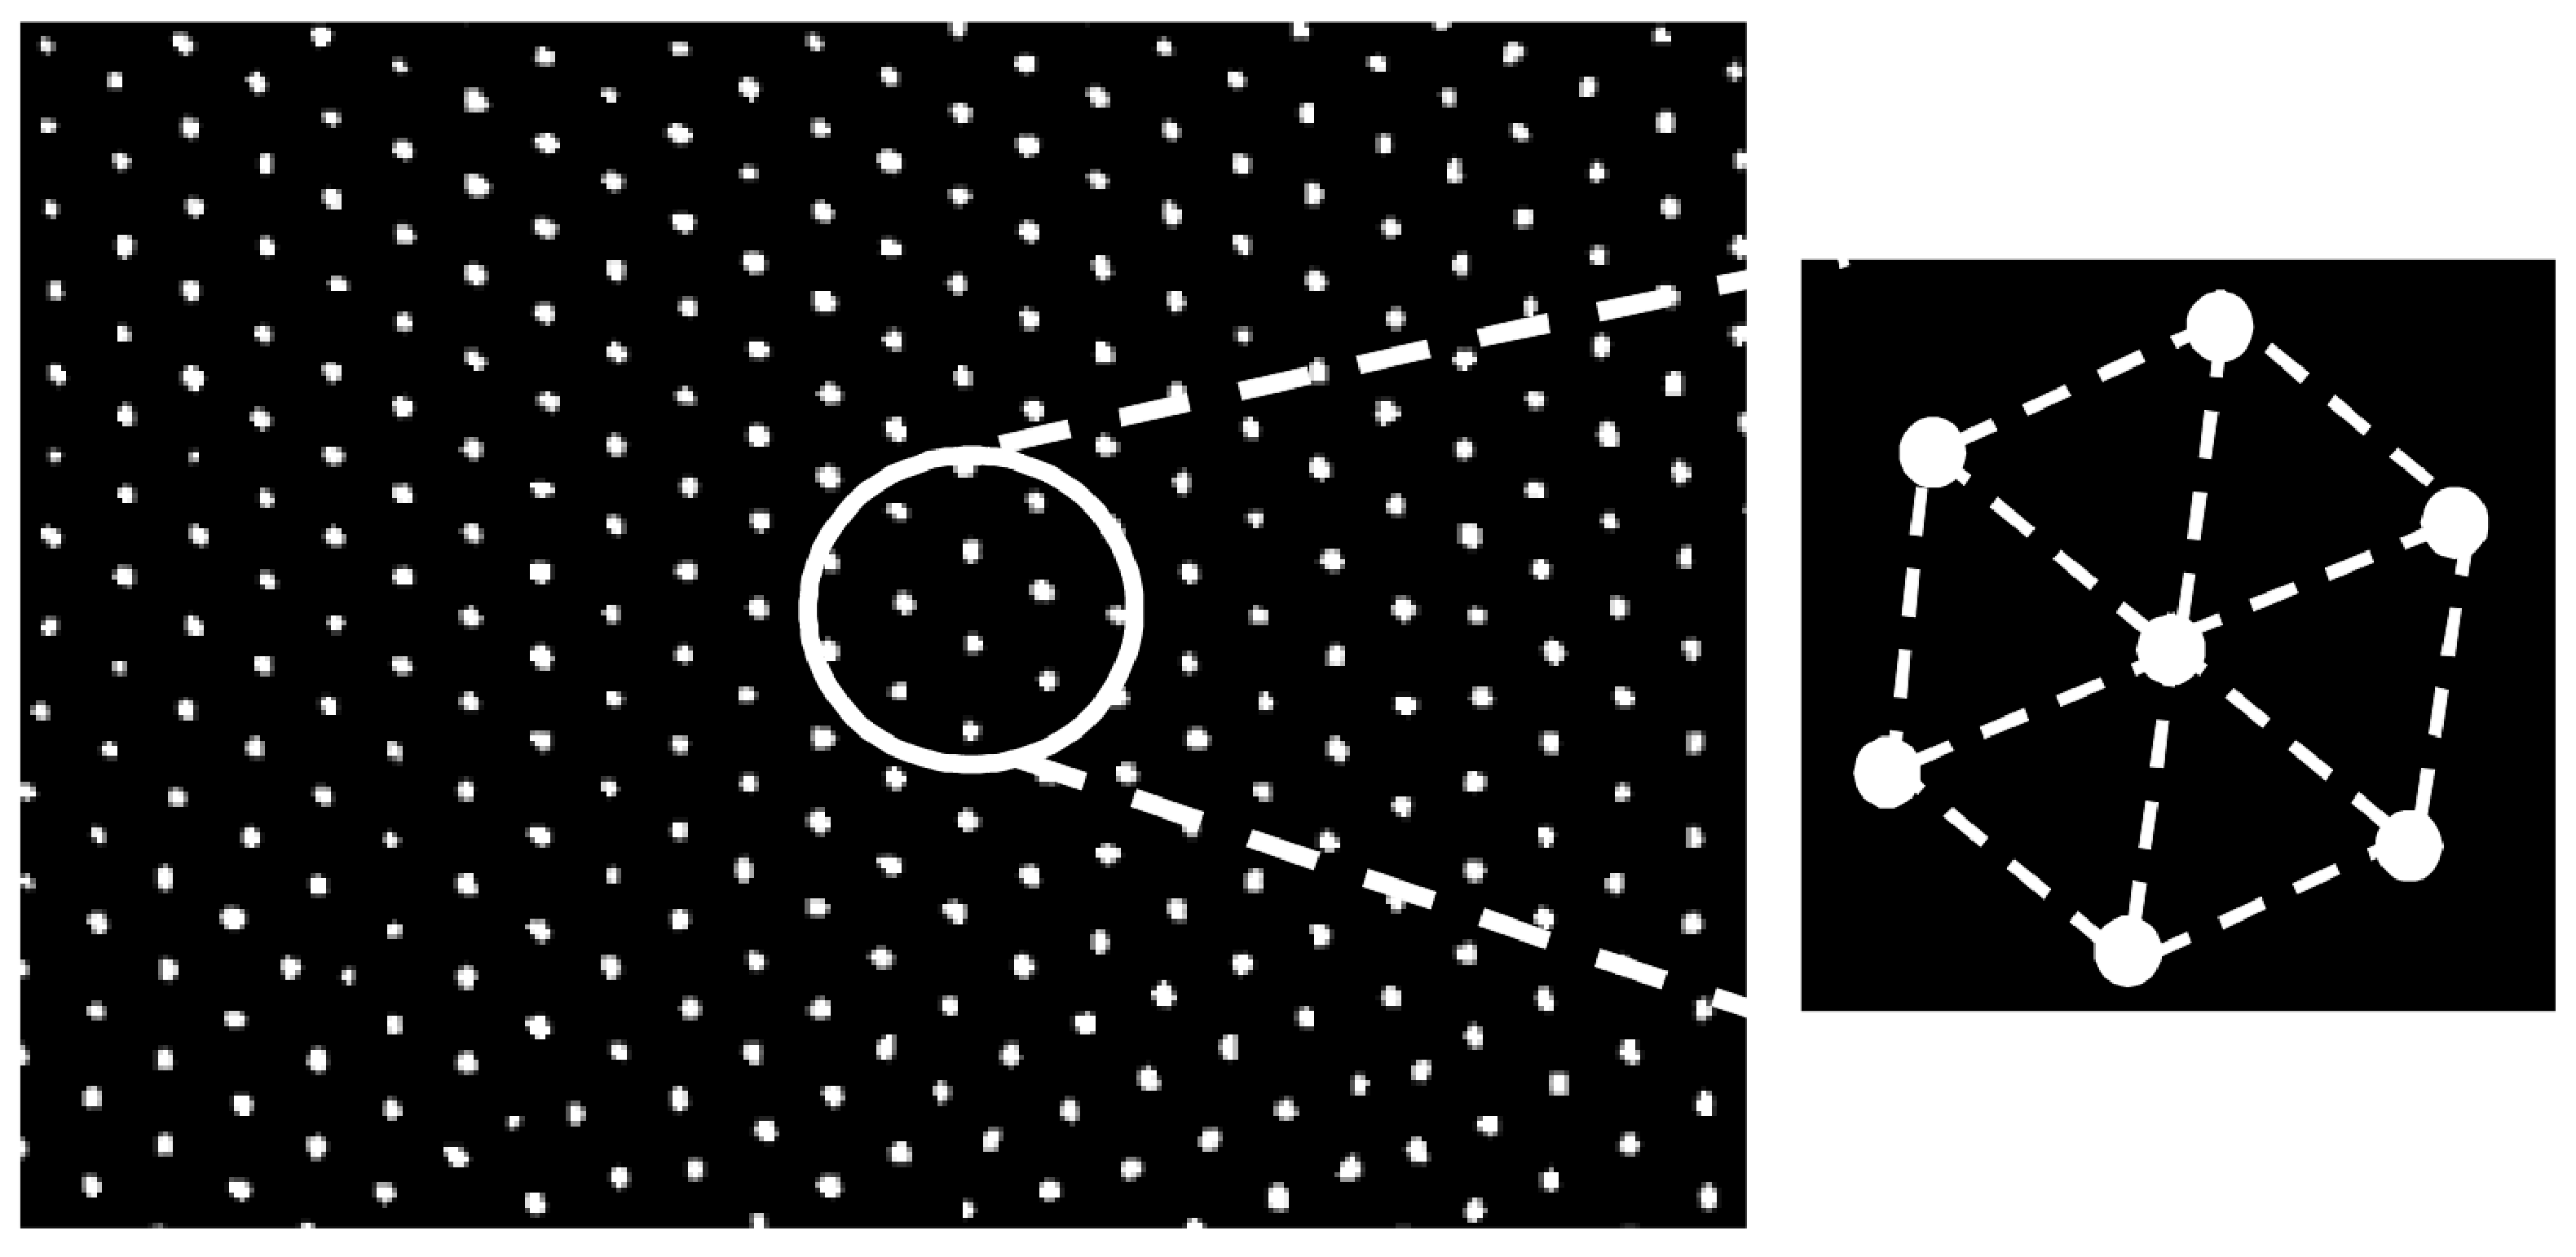
\includegraphics[width=0.9\columnwidth]{figures/eps/coulomb_crystal.eps}
		\caption{2D-s Coulomb kristály képe} 
		\label{fig:measurement} 
	\end{figure}

%----------------------------------------------------------------------------
\section{A mérendő mennyiségek és a származtatott értékek}
%----------------------------------------------------------------------------
	









